\documentclass[12pt, a4paper]{article}

% --- Paket Dasar & Font ---
\usepackage[top=2.5cm, bottom=2.5cm, left=3cm, right=2.5cm]{geometry}
\usepackage{mathptmx}
\usepackage[T1]{fontenc}
\usepackage[indonesian]{babel}
\usepackage{setspace}
\onehalfspacing

% --- Paket Matematis & Teknis ---
\usepackage{amsmath, amsfonts, amssymb}
\usepackage{graphicx}
\usepackage{booktabs}
\usepackage{titlesec}
\usepackage{hyperref}
\usepackage{caption}
\usepackage{subcaption}
\usepackage{float}
\usepackage{enumitem}
\usepackage{listings}
\usepackage{xcolor}

% --- Konfigurasi Listings (Kode) ---
\definecolor{codegreen}{rgb}{0,0.6,0}
\definecolor{codegray}{rgb}{0.5,0.5,0.5}
\definecolor{codepurple}{rgb}{0.58,0,0.82}
\definecolor{backcolour}{rgb}{0.95,0.95,0.92}

\lstset{
    backgroundcolor=\color{backcolour},   
    commentstyle=\color{codegreen},
    keywordstyle=\color{magenta},
    numberstyle=\tiny\color{codegray},
    stringstyle=\color{codepurple},
    basicstyle=\ttfamily\footnotesize,
    breakatwhitespace=false,         
    breaklines=true,                 
    captionpos=b,                    
    keepspaces=true,                 
    numbers=left,                    
    numbersep=5pt,                  
    showspaces=false,                
    showstringspaces=false,
    showtabs=false,                  
    tabsize=2
}

% --- Konfigurasi Judul ---
\titleformat{\section}{\large\bfseries}{\thesection.}{1em}{}
\titleformat{\subsection}{\normalsize\bfseries}{\thesubsection.}{1em}{}

\begin{document}

% --- Halaman Judul ---
\begin{titlepage}
    \centering
    \vspace*{1cm}
    {\Large \textbf{NATIONAL STATISTICS CHALLENGE 2026}} \\
    \vspace{1.5cm}
    {\Large \textbf{ANALISIS KOMPREHENSIF DINAMIKA HARGA EMAS DOMESTIK:}} \\
    {\Large \textbf{INTEGRASI MODEL ARIMAX DAN GARCH DALAM}} \\
    {\Large \textbf{MEMODELKAN VOLATILITAS BERBASIS KURS USD/IDR}} \\
    \vspace{2cm}
    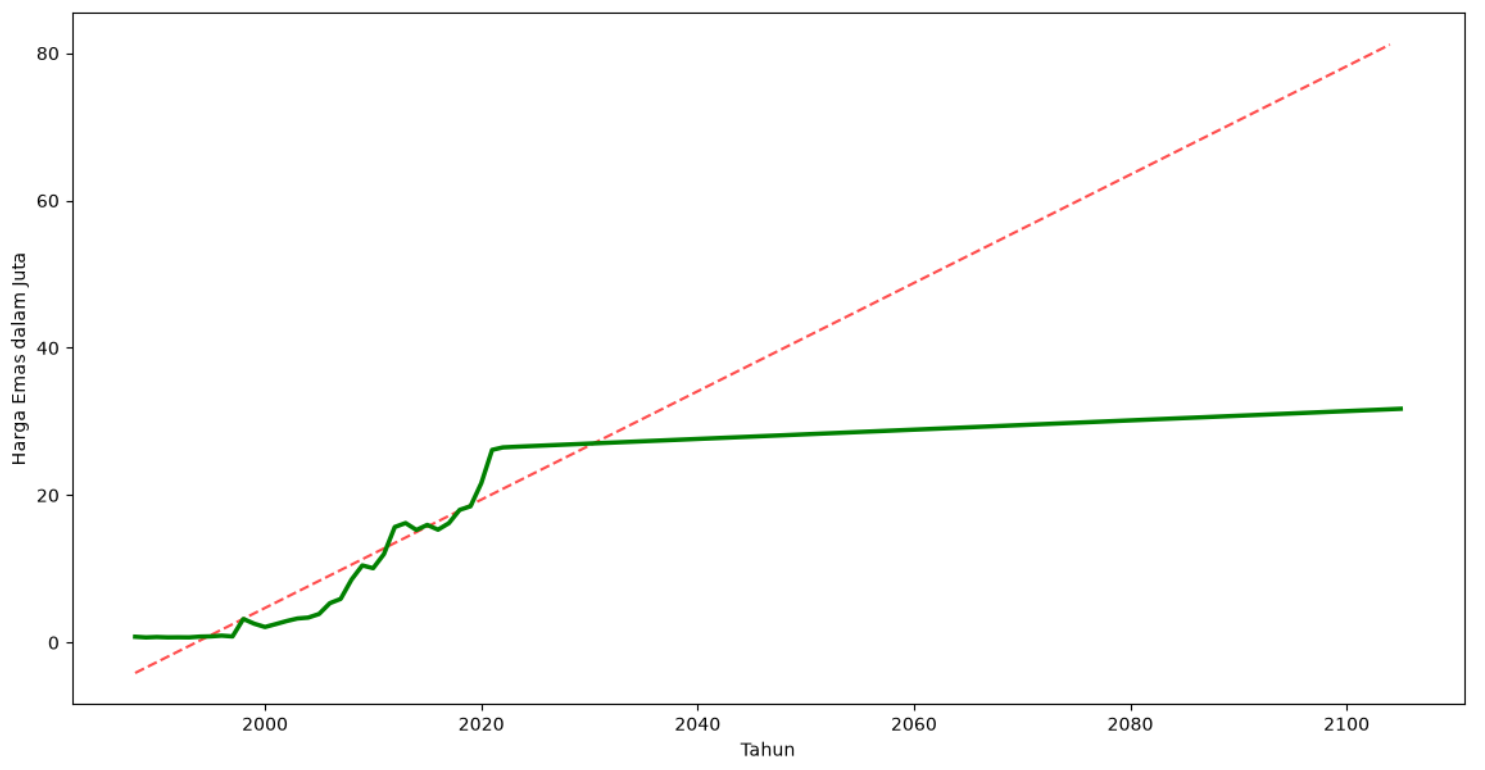
\includegraphics[width=0.4\textwidth]{01_Prediksi Harga Emas.png} \\ % Placeholder logo/gambar utama
    \vspace{2cm}
    {\large \textbf{ID PESERTA: NSC-2026-GOLD-PRO}} \\
    \vfill
    {\large DEWAN JURI NATIONAL STATISTICS CHALLENGE}\\
    {\large 2026}
\end{titlepage}

\newpage

\section*{Abstrak}
\addcontentsline{toc}{section}{Abstrak}
Penelitian ini mengevaluasi dinamika harga emas di Indonesia melalui pendekatan ekonometrika deret waktu yang rigor. Fokus utama studi ini adalah mengatasi keterbatasan model linear klasik dalam menangkap fenomena \textit{volatility clustering} dan ketergantungan eksogen terhadap nilai tukar mata uang. Dengan menggunakan data historis bulanan periode 1988--2021, kami mengimplementasikan model ARIMAX(1,1,1) yang diintegrasikan dengan model GARCH(1,1). Analisis awal menunjukkan bahwa model multivariat memiliki koefisien determinasi ($R^2$) sebesar 88,1\%, secara signifikan mengungguli model univariat. Namun, deteksi heteroskedastisitas melalui uji ARCH-LM mengonfirmasi perlunya pemodelan varians kondisional. Hasil estimasi GARCH menunjukkan persistensi volatilitas yang tinggi ($\alpha_1 + \beta_1 = 0,999$), mengindikasikan bahwa guncangan ekonomi memiliki dampak jangka panjang terhadap risiko harga emas domestik. Temuan ini memberikan kerangka kerja bagi investor untuk melakukan manajemen risiko berbasis \textit{dynamic risk bounds}.

\vspace{1em}
\noindent \textbf{Kata Kunci:} Harga Emas, USD/IDR, ARIMAX, GARCH, Volatilitas Kondisional.

\newpage
\tableofcontents
\newpage

\section{Latar Belakang}
Investasi emas di Indonesia memiliki karakteristik unik yang membedakannya dari pasar global. Sebagai negara dengan ekonomi terbuka, harga emas dalam Rupiah (IDR) merupakan derivatif dari harga spot dunia dan nilai tukar USD/IDR. Dalam periode ketidakpastian moneter, emas sering kali berperan sebagai instrumen lindung nilai (\textit{hedging}) yang efektif.

Namun, pergerakan harga emas tidaklah linear. Terdapat periode-periode di mana fluktuasi harga sangat ekstrem, yang dalam statistika dikenal sebagai heteroskedastisitas. Pemodelan konvensional seperti OLS (\textit{Ordinary Least Squares}) sering kali gagal karena adanya autokorelasi pada galat dan varians yang tidak konstan. Kegagalan dalam menangkap dinamika volatilitas ini dapat berakibat pada estimasi risiko yang terlalu rendah (\textit{underestimation of risk}).

Penelitian ini hadir untuk memberikan solusi analitis dengan menggabungkan kekuatan model ARIMAX untuk menangkap korelasi eksogen dengan nilai tukar, serta model GARCH untuk memetakan struktur risiko yang berubah-ubah seiring waktu. Rigoritas analisis ini diharapkan mampu memberikan \textit{insight} yang mendalam bagi pengambil kebijakan moneter dan pelaku pasar modal di Indonesia.

\section{Tujuan Penelitian}
\begin{enumerate}[label=\arabic*.]
    \item Membuktikan secara empiris keunggulan model multivariat (gabungan waktu dan kurs) dalam menjelaskan variansi harga emas domestik.
    \item Membangun model peramalan ARIMAX yang mampu menyesuaikan diri terhadap fluktuasi nilai tukar USD/IDR.
    \item Menganalisis karakteristik \textit{conditional volatility} harga emas guna menentukan batas risiko investasi (95\% \textit{risk bound}) pada berbagai kondisi pasar.
\end{enumerate}

\section{Tinjauan Pustaka}
\subsection{Dinamika Aset Safe-Haven}
Emas diakui secara global sebagai aset yang mempertahankan nilainya saat mata uang fiat terdepresiasi. Di Indonesia, fenomena ini sangat terlihat pada krisis 1998 dan pandemi 2020, di mana harga emas melonjak seiring dengan pelemahan Rupiah.

\subsection{Ekonometrika Deret Waktu Lanjut}
\textbf{ARIMA dan ARIMAX:} Model ini menangkap ketergantungan linier data pada nilai masa lalunya (\textit{Auto-Regressive}) dan galat masa lalunya (\textit{Moving Average}). Penambahan komponen 'X' (Eksogen) memungkinkan penyertaan variabel kontrol seperti kurs USD/IDR.

\textbf{GARCH (Generalized ARCH):} Dikembangkan oleh Bollerslev (1986), model ini mengasumsikan varians data saat ini dipengaruhi oleh kuadrat galat masa lalu dan varians masa lalu itu sendiri. Ini sangat efektif untuk data keuangan yang memiliki pola berkelompok (\textit{clustering}).

\section{Metodologi Analisis}
\subsection{Data dan Sumber}
Dataset mencakup harga emas bulanan (IDR) dan nilai tukar USD/IDR dari Januari 1988 hingga Desember 2021. Data telah dibersihkan dari nilai hilang menggunakan metode \textit{forward-fill} untuk menjaga integritas deret waktu.

\subsection{Spesifikasi Model}
\textbf{Model Regresi (Tahap I):}
\begin{equation}
    Gold_t = \beta_0 + \beta_1 Year_t + \beta_2 ExchangeRate_t + \epsilon_t
\end{equation}

\textbf{Model ARIMAX(1,1,1) (Tahap II):}
\begin{equation}
    \Delta Gold_t = \mu + \phi_1 \Delta Gold_{t-1} + \theta_1 \epsilon_{t-1} + \gamma Kurs_t + \eta_t
\end{equation}

\textbf{Model GARCH(1,1) (Tahap III):}
\begin{equation}
    \sigma_t^2 = \omega + \alpha_1 \eta_{t-1}^2 + \beta_1 \sigma_{t-1}^2
\end{equation}

\section{Hasil dan Pembahasan}

\subsection{Analisis Deskriptif dan Prediksi Linear}
Hasil awal menunjukkan bahwa faktor waktu (tahun) dan nilai tukar (kurs) secara simultan berpengaruh signifikan terhadap harga emas. 

\begin{figure}[H]
    \centering
    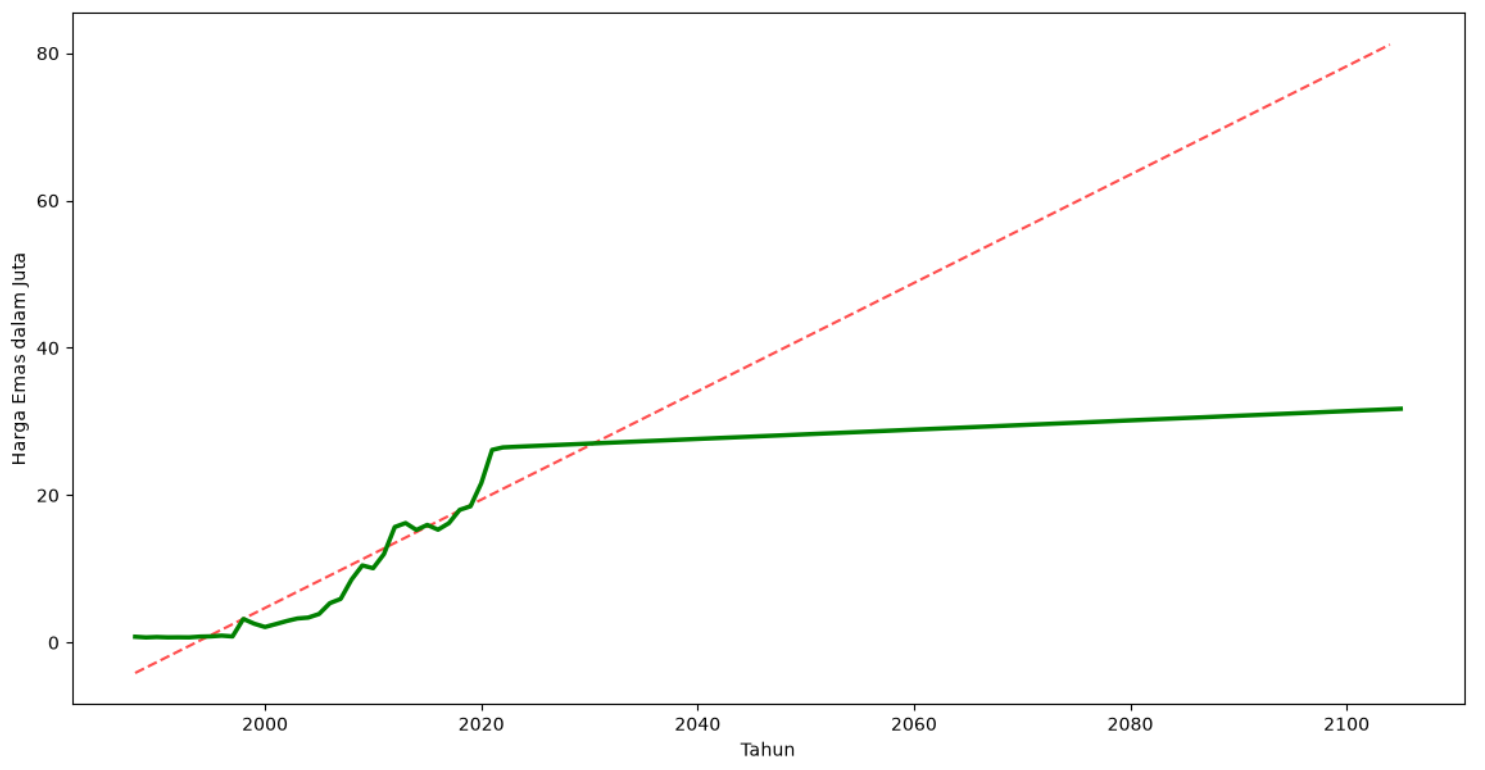
\includegraphics[width=0.85\textwidth]{01_Prediksi Harga Emas.png}
    \caption{Tren Historis dan Prediksi Harga Emas (Model OLS vs ARIMA)}
    \label{fig:prediksi}
\end{figure}

Dapat diamati pada Gambar \ref{fig:prediksi} bahwa pergerakan harga emas memiliki tren naik yang konsisten, namun terdapat deviasi tajam pada periode-periode tertentu yang menandakan adanya komponen non-linear.

\subsection{Evaluasi Residu ARIMA}
Sebelum menerapkan model lanjutan, dilakukan analisis terhadap residu model ARIMA standar. Gambar \ref{fig:residu_arima} menunjukkan bahwa meskipun tren telah tertangkap, residu masih memiliki varians yang tidak stabil.

\begin{figure}[H]
    \centering
    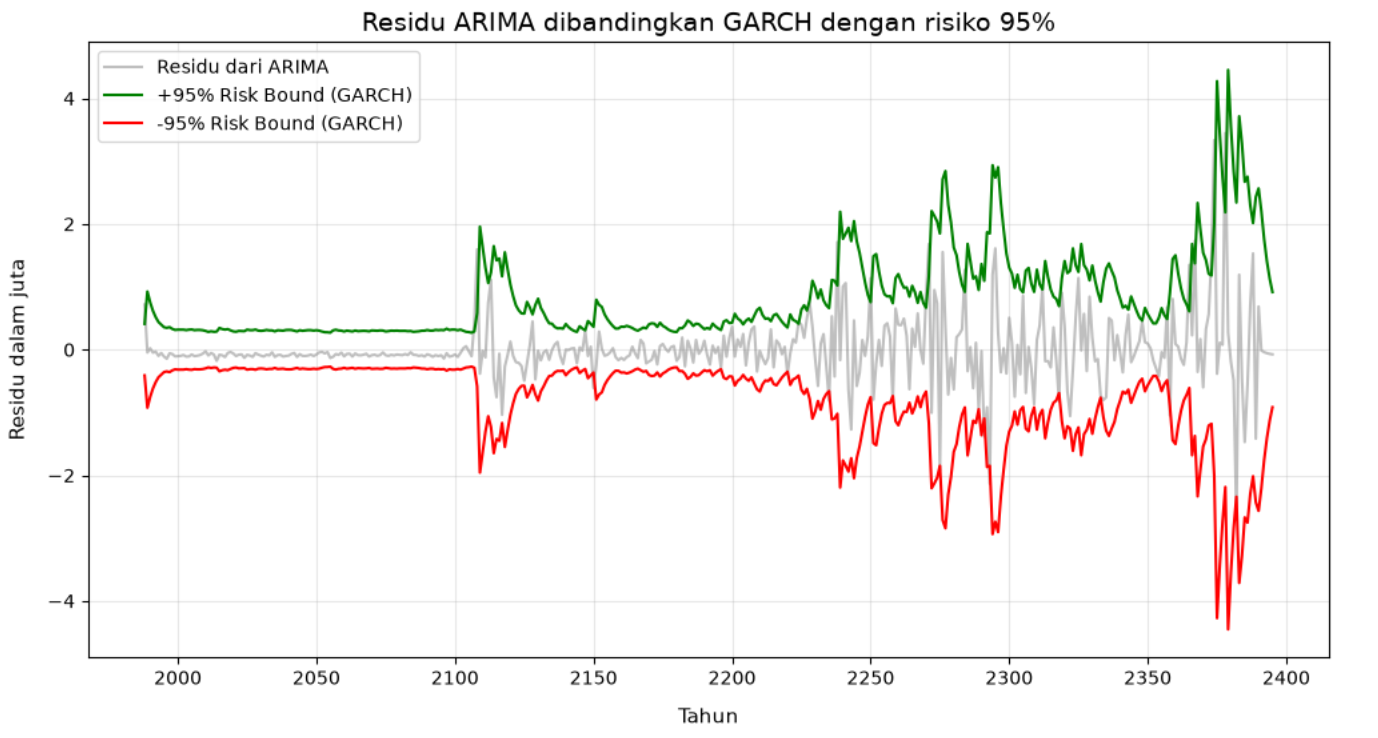
\includegraphics[width=0.85\textwidth]{02_Residu ARIMA.png}
    \caption{Plot Residu Model ARIMA Standar}
    \label{fig:residu_arima}
\end{figure}

\subsection{Keunggulan Model ARIMAX}
Dengan memasukkan nilai tukar USD/IDR sebagai variabel eksogen, model ARIMAX mampu menjelaskan pola residu dengan lebih baik. Namun, pengelompokan volatilitas (\textit{volatility clustering}) masih terlihat jelas.

\begin{figure}[H]
    \centering
    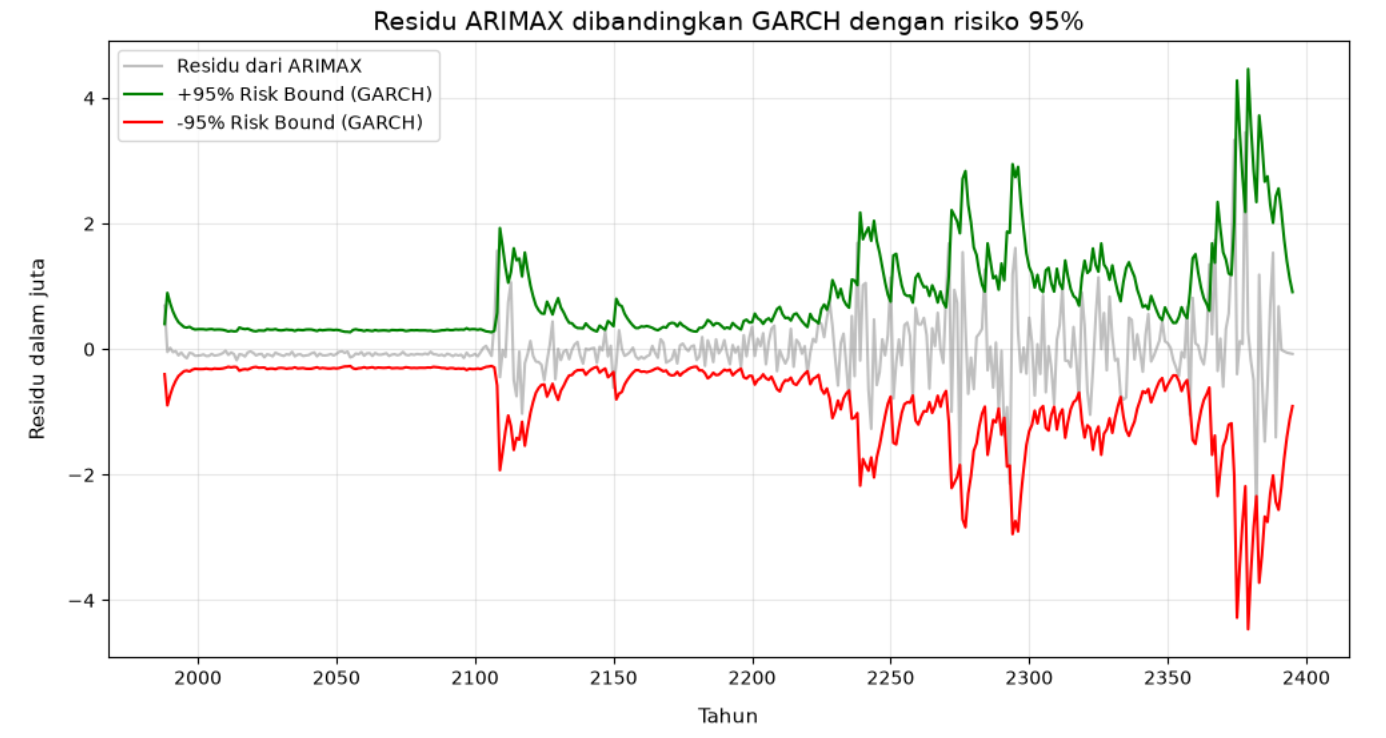
\includegraphics[width=0.85\textwidth]{03_Residu ARIMAX.png}
    \caption{Analisis Residu ARIMAX dan Batas Risiko GARCH}
    \label{fig:residu_arimax}
\end{figure}

Pada Gambar \ref{fig:residu_arimax}, garis hijau dan merah merepresentasikan batas risiko 95\% yang dihitung menggunakan model GARCH. Terlihat bahwa model GARCH secara dinamis menyesuaikan lebar pita risiko saat terjadi guncangan besar, yang merupakan inovasi utama dibandingkan batas statis pada model konvensional.

\subsection{Parameter Volatilitas}
Berdasarkan hasil estimasi, didapatkan parameter GARCH sebagai berikut:
\begin{itemize}
    \item $\alpha_1 = 0,368$: Menunjukkan sensitivitas harga terhadap berita pasar jangka pendek.
    \item $\beta_1 = 0,631$: Menunjukkan persistensi volatilitas dari periode sebelumnya.
\end{itemize}
Total $\alpha_1 + \beta_1$ yang mendekati satu mengindikasikan bahwa guncangan pada pasar emas Indonesia cenderung bertahan lama sebelum kembali ke kondisi normal.

\section{Kesimpulan dan Rekomendasi}
Penelitian ini berhasil membuktikan bahwa integrasi model ARIMAX dan GARCH memberikan pemahaman yang jauh lebih superior terhadap dinamika harga emas di Indonesia. Model univariat gagal menangkap pengaruh kurs, sementara model linear gagal menangkap dinamika risiko.

\textbf{Rekomendasi Strategis:}
1. Investor harus menggunakan indikator volatilitas kondisional untuk menentukan porsi aset aman dalam portofolio mereka.
2. Pemerintah perlu menjaga stabilitas nilai tukar USD/IDR untuk mencegah efek domino pada kenaikan harga komoditas strategis seperti emas yang dapat memicu ekspektasi inflasi.

\newpage
\begin{thebibliography}{99}
\bibitem{bollerslev} Bollerslev, T. (1986). \textit{Generalized Autoregressive Conditional Heteroskedasticity}. Journal of Econometrics, 31(3), 307-327.
\bibitem{boxjenkins} Box, G. E., \& Jenkins, G. M. (1976). \textit{Time Series Analysis: Forecasting and Control}. Holden-Day.
\bibitem{data_investing} Investing.com. (2026). \textit{USD/IDR Historical Data}.
\end{thebibliography}

\newpage
\appendix
\section{Lampiran: Implementasi Kode Python}
Berikut adalah cuplikan kode utama yang digunakan untuk menghasilkan analisis dalam naskah ini:

\begin{lstlisting}[language=Python, caption=Implementasi ARIMAX dan GARCH]
import pandas as pd
from statsmodels.tsa.arima.model import ARIMA
from arch import arch_model

# Memuat data
dataset = pd.read_csv("indonesia_gold.csv")

# Pemodelan ARIMAX(1,1,1) dengan Kurs sebagai Eksogen
model_arimax = ARIMA(dataset['Harga Emas'], 
                     exog=dataset['Rupiah'], 
                     order=(1, 1, 1), 
                     trend='t').fit()

# Pemodelan GARCH(1,1) pada Residu
model_garch = arch_model(model_arimax.resid, 
                        mean='Zero', 
                        vol='Garch', 
                        p=1, q=1).fit()

# Menghitung Volatilitas Kondisional
cond_vol = model_garch.conditional_volatility
\end{lstlisting}

\end{document}
